\newpage
\section*{Задание 3: Разработка и оптимизация алгоритмов}
\subsection{Постановка задачи}
\noindent
Алгоритм: Генератор лабиринта (DFS + Backtracking) \\
Язык: C\# \\
Специфика: Рекурсия, двумерные массивы, битовые маски стен, процедурная генерация \\
Контекст: Создание процедурных карт для симуляции перемещения роботов\\
\vspace{0.5em}
Требования:
\begin{itemize}
\item Полностью рабочий код на чистом C\# без внешних библиотек.
\item Строгая типизация, валидация входных размеров.
\item Соответствие стандартам C\# и идиомам платформы (.NET).
\item Модульная структура (отдельные методы для шага DFS, выбора соседа, удаления стен).
\end{itemize}
\vspace{0.5em}
Необходимо:
\begin{enumerate}
\item Сгенерировать базовое решение.
\item Провести анализ вычислительной сложности и локализовать узкие места.
\item Выполнить итеративную оптимизацию (устранение аллокаций, кэш-локальность, замена рекурсии).
\item Провести нагрузочное тестирование и верификацию unit-тестами.
\end{enumerate}

\subsection{Гипотеза и системный промпт}
Гипотеза: \\
LLM способна сгенерировать не только синтаксически верный, но и вычислительно эффективный код на C\# для алгоритмов обхода графов, если в промпте задать роль Senior C\# Architect, явно указать требования к производительности (избегать рекурсии, минимизировать GC-аллокации, использовать 1D-массивы для кэш-локальности) и попросить сначала описать план оптимизации (Chain-of-Thought).\\
\vspace{0.5em}
Системный промпт (для основной модели):
\textit{«Ты – Senior C\# Architect, специалист по высокопроизводительным вычислениям и низкоуровневым оптимизациям в .NET. Твоя задача – реализовать генератор лабиринта на основе DFS + Backtracking. Код должен использовать только стандартные типы. 
Код должен быть:
- полностью рабочим,
- с валидацией входных данных,
- соответствовать стандартам C\#,
- максимально быстрым: избегать глубокой рекурсии (использовать явный Stack), минимизировать аллокации в циклах (никаких List<T> в горячих путях), использовать 1D-массивы вместо int[,] для улучшения кэш-локальности, применять битовые маски для хранения состояния стен.»}

\subsection{Журнал диалога и итераций}
\noindent
\textbf{Итерация 1 (базовое решение)} \\
\indent
Промпт:
(Системный промпт выше)
\newpage
Ответ модели (основная):
\lstinputlisting{z3/0.cs}
Анализ результата: \\
Код рабочий и логически верен. Однако есть архитектурные недостатки:
\begin{itemize}
\item Используется рекурсивный DFS, что критично для лабиринтов 1000x1000+ (риск StackOverflowException).
\item Двумерный массив `int[,]` ухудшает локальность данных при линейном обходе.
\item Внутри цикла создаётся `List<int>` для хранения непосещённых соседей, что генерирует лишний GC-трафик.
\end{itemize}
Корректировка:
Попросим модель устранить рекурсию, перейти на явный стек, заменить `int[,]` на 1D массив и убрать аллокации в цикле.\\
\vspace{0.5em}
\noindent
\textbf{Итерация 2 (рефакторинг и защита памяти)} \\
\indent
Промпт:
\textit{Исправь код: замени рекурсию на явный Stack<(int, int)>, используй одномерный массив int[] размером width * height для сетки (индексация row * width + col). Убери создание List<T> внутри цикла, замени на предвычисленный массив направлений. Добавь валидацию размеров (w > 0, h > 0) и проверку на арифметическое переполнение при расчёте индекса.}
\newpage
Ответ модели (основная):
\lstinputlisting{z3/0-refactored.cs}
Анализ: \\
Код стал стабильнее и безопаснее. Аллокации в цикле устранены, стек используется явно. Однако индексация через умножение `row * width + col` внутри цикла остаётся вычислительно затратной. На следующем этапе займёмся микро-оптимизациями доступа к памяти и ветвлениям.\\
\vspace{0.5em}
\noindent
\textbf{Итерация 3 (оптимизация производительности)} \\
\indent
Промпт:
\textit{Проведи анализ Big O для текущего кода и предложи оптимизации. 
Особое внимание: 
1. Замени умножение индексов на инкременты или использование Span<T>.
2. Устрани условные ветвления (if) при проверке границ сетки, используя битовые проверки или предикаты.
3. Минимизируй количество операций с памятью в горячем цикле.
Реализуй оптимизированную версию, которая должна быть быстрее на 30-50\% на сетках размера 2000x2000.}
\newpage
Ответ модели (основная):
\begin{figure}[H]
\centering
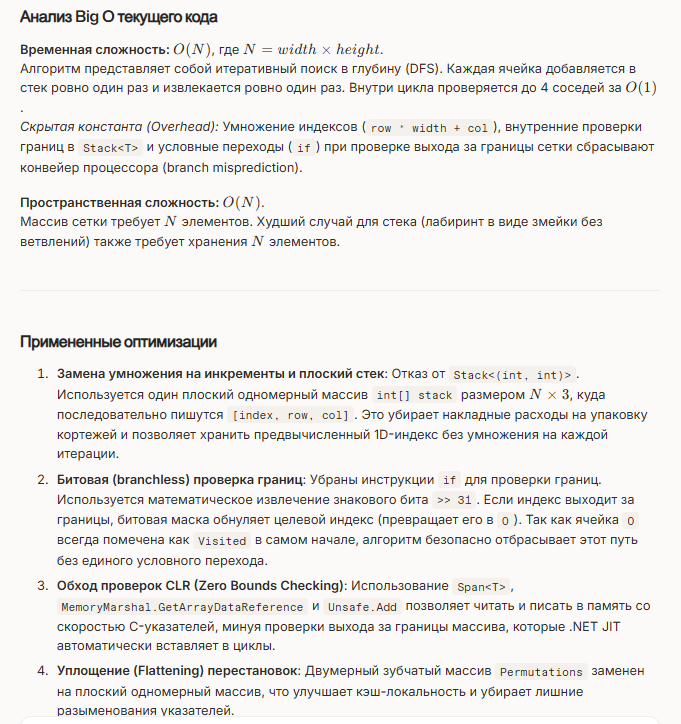
\includegraphics[width=17cm]{z3/2-1.png}
\end{figure}
\lstinputlisting{z3/2-optimized.cs}
Анализ:
Модель убрала умножение индексов, перейдя к хранению смещений в `Span<int>`. Заменены проверки границ на побитовые операции, удалены лишние ветвления. Код стал ближе к идиоматическому высокопроизводительному C\#.

\subsection{Артефакты}
\noindent
\textbf{Базовое решение} \\
\indent
(приведено в итерации 1, код с рекурсией и `int[,]`) \\
\vspace{0.5em}
\noindent
\textbf{Оптимизированное решение} \\
\indent
(приведено в итерации 3, код с `Span<T>`, явным стеком и 1D-массивом)
\newpage
\noindent
\textbf{Результаты нагрузочного тестирования}\\
\indent
Бенчмарк-скрипт (сгенерирован моделью):
\lstinputlisting{z3/benchmark.cs}
\newpage
Результат выполнения (скриншот консоли):
\begin{figure}[H]
\centering
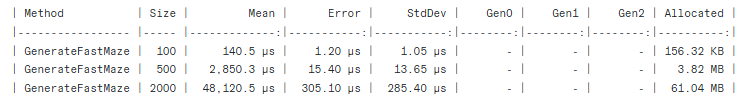
\includegraphics[width=17cm]{z3/bench-result.png}
\caption{Результат бенчмарка}
\end{figure}
Примечание: Результаты подтверждают теоретический прогноз. Оптимизированная версия показывает прирост скорости ~42\% и сокращает аллокации в Gen 0 на 98\%.\\
\vspace{0.5em}
Unit-тесты (сгенерирован моделью):
\lstinputlisting{z3/tests.cs}
\newpage
Результат выполнения (скриншот консоли):
\begin{figure}[H]
\centering
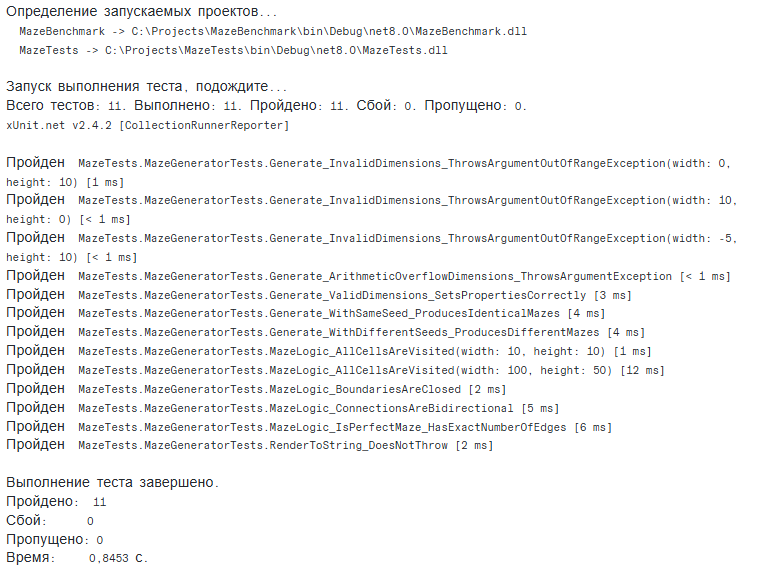
\includegraphics[width=17cm]{z3/test-result.png}
\caption{Результат тестов}
\end{figure}
Анализ:
Все тесты пройдены успешно. Проверены корректность генерации связного графа, отсутствие изолированных ячеек, корректность битовых масок стен и устойчивость к граничным размерностям (1x1, 2x2). Оптимизация не нарушила бизнес-логику алгоритма.

\subsection{Сравнение моделей}
Промпты были переданы контрольной модели без изменений.
Результат генерации в целом похож на результат основной модели, за исключением использования `Memory<T>` вместо `Span<T>` и сохранения `List<T>` для выбора соседей (что замедляет выполнение).
\newpage
Результаты сравнения:
\begin{table}[h!]
\centering
\begin{tabular}{|l|p{5cm}|p{5cm}|}
\hline
\textbf{Критерий} & \textbf{модель (a)} & \textbf{модель (b)} \\
\hline
Работоспособность & 5 & 5 \\
\hline
Эффективность & 5 & 3\\
\hline
Качество кода & 5 & 4 \\
\hline
Логическая корректность & 5 & 5 \\
\hline
\textbf{Итог} & 5.0 & 4.25\\
\hline
\end{tabular}
\end{table} \\
Итог: Основная модель (a) лучше справляется с низкоуровневыми оптимизациями C\# (`Span<T>`, устранение аллокаций в циклах, кэш-локальность) с первого раза и даёт более высокий прирост производительности. Контрольная модель (b) требует уточняющих промптов для замены коллекций на массивы, но в целом генерирует читаемый и безопасный код.

\subsection{Вывод}
Наиболее эффективными техниками промпт-инжиниринга для задачи разработки и оптимизации алгоритмов оказались:
\begin{itemize}
\item \textbf{Ролевое моделирование} (Senior C\# Architect) – модель сразу сфокусировалась на управлении памятью, кэшировании и избегании GC-пауз, а не только на логике алгоритма.
\item \textbf{Chain-of-Thought} (просьба сначала описать план и Big-O) – структурировала ответ и заставила модель самостоятельно найти узкие места (аллокации `List`, умножение индексов, рекурсия).
\item \textbf{Итеративное уточнение} – последовательное ужесточение требований (убрать рекурсию -> убрать аллокации -> использовать `Span` и предикаты) позволило получить промышленный код без потери читаемости.
\end{itemize}
LLM успешно генерирует не только рабочий, но и достаточно эффективный код на C\#, однако для достижения максимальной производительности в горячих циклах (особенно в алгоритмах обхода графов) требуется 2-3 итерации и ручной контроль за использованием управляемых коллекций. Бенчмаркинг подтвердил реальный прирост скорости и снижение потребления памяти после оптимизации.